\section{Simulation}
\label{sec:Simulation}

\subsection{Detector Description for High Energy Physics}
We used Detector Description for High Energy Physics (DD4hep) standalone version.
DD4hep is a software framework to provide overall detector description for experiments.
It offers a consistent description through a single source of detector information for simulation, reconstruction, analysis, etc.
Additionally, DD4hep being developed for high luminosity large hadron collider (HL-LHC) detector simulation.
During the internship, we built the geometry of CODEX-b constructing hierachy system.
We designed concrete shield wall to block particles from particle gun or MC and herschel detector since we used as a scintillator for our measurement.
For validation $\mu$ particle gun and minbias event had been used.
We also checked energy deposits and positions of CODEX-b hits. 

%I learn how to make geometry: layer, station, super staion, envelope (hierachy).
%I define materials for our detector and CODEX-b geometry such as concrete, Herschel detector.
%Layer consists of silicon, station consists of aluminum. 
%There is a veto cone with two lead and one silicon. 
%Also just in front of CODEX-b, concrete wall exists to veto muons.
%First of all, using muon particle gun with high energy, test our geometry.
%And then using HepMC to generate pp collisions and do the same process as muon particle gun.
%I made hierachy system to build CODEX-b (envelop, super station, station, layer).
%I could check energy deposits and positions of CODEX-b hits.

\subsection{Simulation geometry}
First geometry is the CODEX-b.
CODEX-b consists of two parts face station and inner station.
Based on the paper, face station has 6 resistive plate chambers (RPCs) layers at 4~cm intervals with 1~cm granularity.
The size of each layer is 10 x 10~$m^{2}$ and the thickness is 2~cm. 
In this simulation we had been implemented layers as a tracker instead of RPCs.
Inner station also has same configuration except number of layers.
It will be equally spaced with triplets along the depth to minimize distance between reconstructed vertex and 1st measurement. 

%To make coincidence setup with test-bench, I made two Herschel plates with the same positions where all equipment have set.
%Two plates with 30 x 30~$cm^{2}$ size, 2~cm thickness.
%There is a concrete wall in front of scintillators.
%3~m thickness to suppress particles from pp collisions.
%Roughly in 1000 events, it has hits on scinitillators 4 - 9 events.
%There is a proposed veto cone. It consists of two lead absorbers and one silicon tracker.
%There is also concrete wall which blocks radiations (or particles) to reach CODEX-b box. 
%It has 3.2~m thickness.

\begin{figure}[h]
\begin{center}
  \begin{tabular}[t]{cc}
    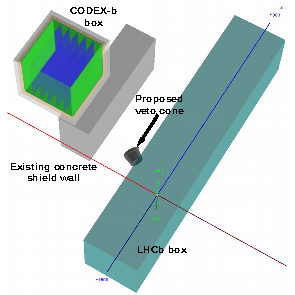
\includegraphics[width=0.5\textwidth]{figs/INT/CODEXbBigGeo.pdf} &
    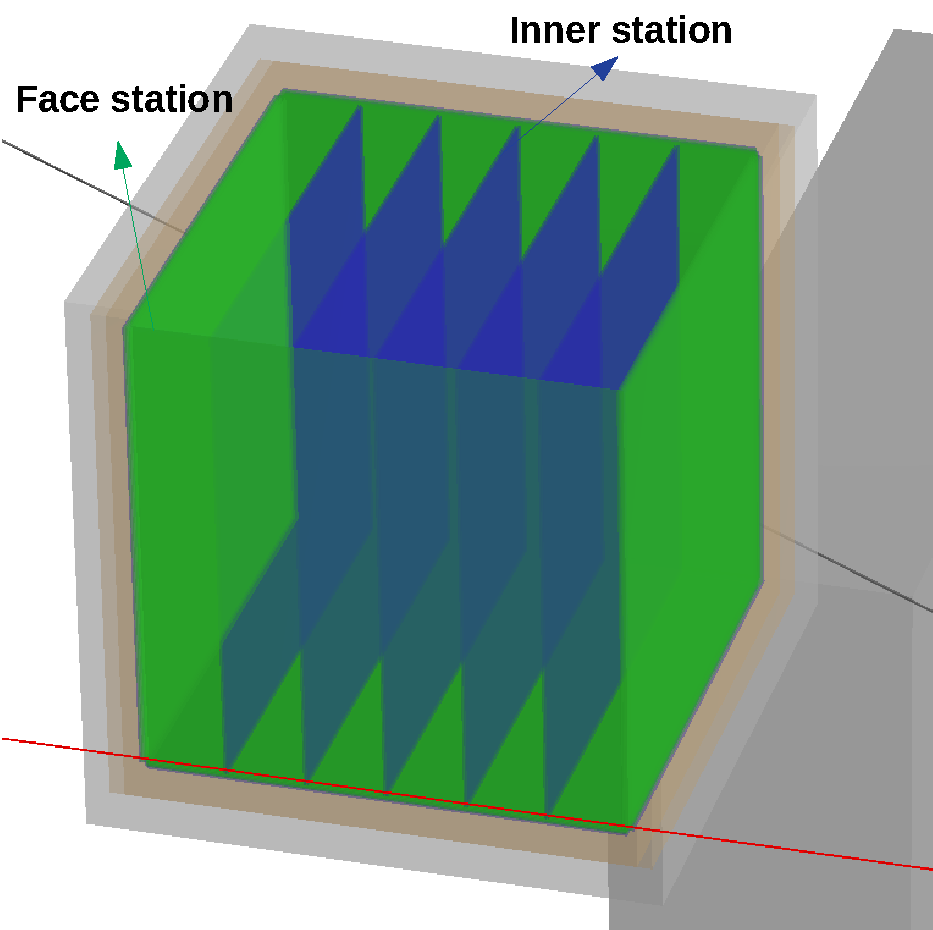
\includegraphics[width=0.5\textwidth]{figs/INT/ZoomVersion.pdf}
  \end{tabular}
\end{center}
\caption{
    Wide view of CODEX-b simulation geometry
}
\end{figure}

We also created a concrete shield wall with 3.2~m thickness.
It was placed just front of CODEX-b box.
Between the LHCb box and the concrete wall, there is a proposed veto cone.
It contains two lead absorber and one active silicon layer.

\subsection{Simulation status}

We designed two different detectors based on similar geometry, one is the CODEX-b and the other is scintillator.
Both were tested with $\mu$ particle gun with 1\tev and the minimum bias events generated from the standalone Gauss. 

\begin{figure}[h]
\centering
    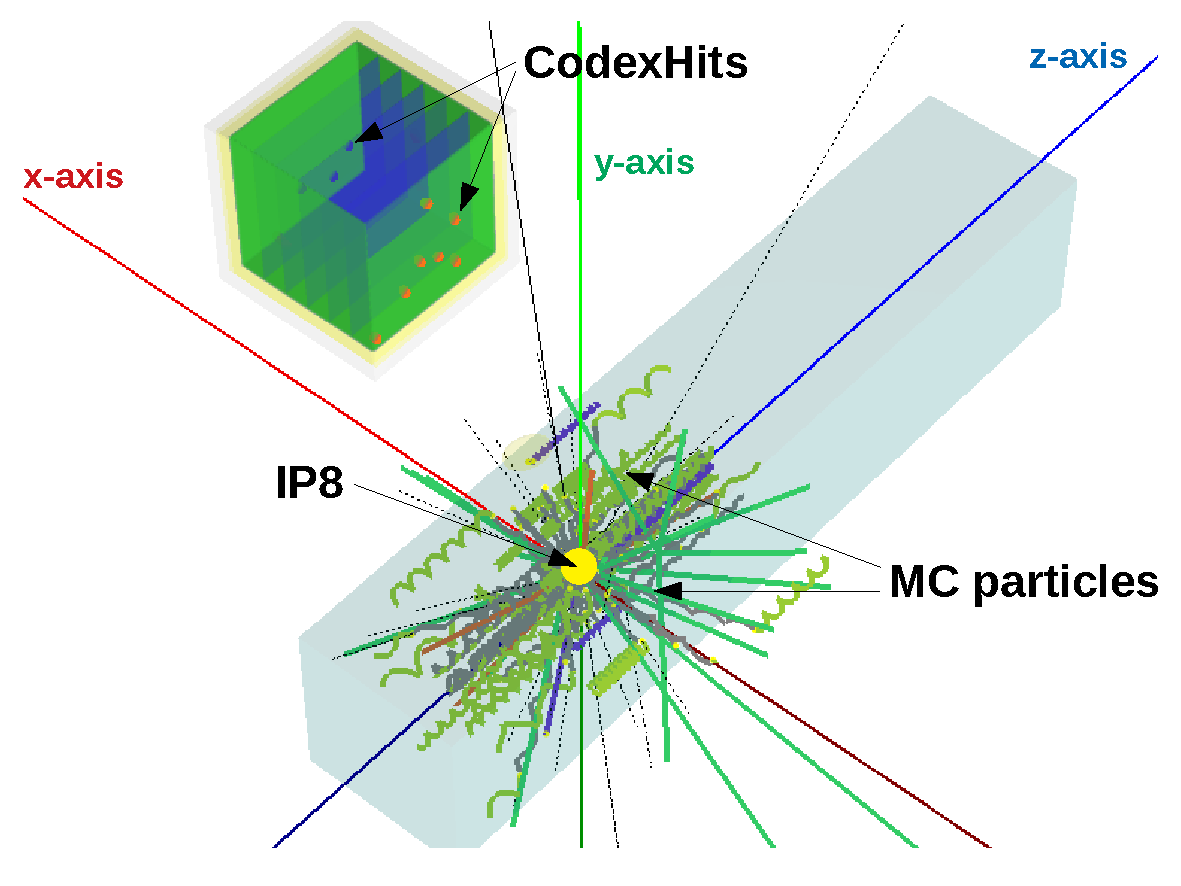
\includegraphics[width=12cm]{figs/INT/Minbias.pdf} \\
    \vspace{0.25cm} 
    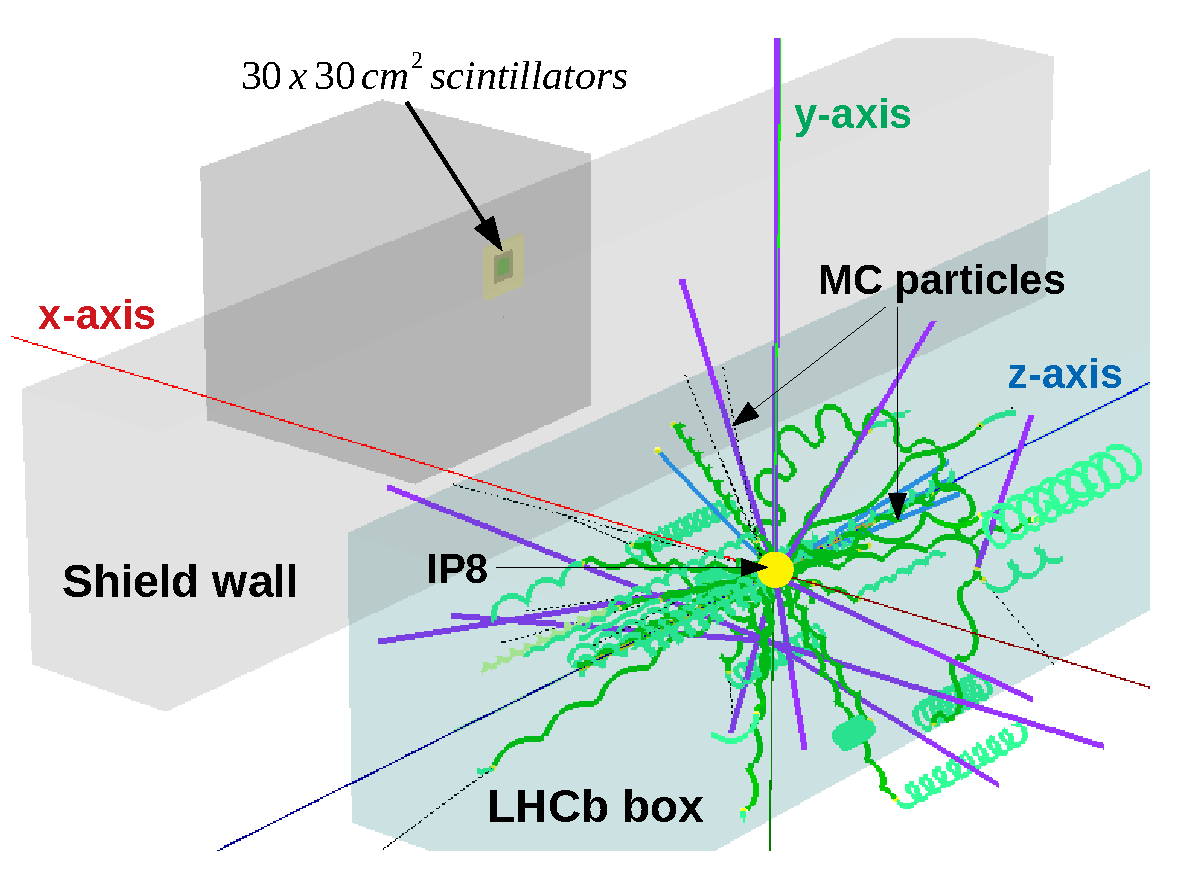
\includegraphics[width=12cm]{figs/INT/Scint.pdf}
\caption{
    Validation of the CODEX-b simulation by removing the concrete shield wall with minimum bias events 
}
\end{figure}

%\begin{figure}[h]
%\centering
%\caption{
%    Test of the scintialltor configuration with minimum bias events
%}
%\end{figure}
